

% Gradient Info
  
\tikzset {_yf8nxye1j/.code = {\pgfsetadditionalshadetransform{ \pgftransformshift{\pgfpoint{9.5 bp } { 15.5 bp }  }  \pgftransformscale{1 }  }}}
\pgfdeclareradialshading{_r90b3jz8c}{\pgfpoint{0bp}{0bp}}{rgb(0bp)=(1,1,1);
rgb(0bp)=(1,1,1);
rgb(25bp)=(0.82,0.01,0.11);
rgb(400bp)=(0.82,0.01,0.11)}

% Gradient Info
  
\tikzset {_nifyjqsrp/.code = {\pgfsetadditionalshadetransform{ \pgftransformshift{\pgfpoint{9.5 bp } { 15.5 bp }  }  \pgftransformscale{1 }  }}}
\pgfdeclareradialshading{_dfo8mv0ol}{\pgfpoint{0bp}{0bp}}{rgb(0bp)=(1,1,1);
rgb(0bp)=(1,1,1);
rgb(25bp)=(0.82,0.01,0.11);
rgb(400bp)=(0.82,0.01,0.11)}

% Gradient Info
  
\tikzset {_fal5ao0nl/.code = {\pgfsetadditionalshadetransform{ \pgftransformshift{\pgfpoint{9.5 bp } { 15.5 bp }  }  \pgftransformscale{1 }  }}}
\pgfdeclareradialshading{_6z78fwt66}{\pgfpoint{0bp}{0bp}}{rgb(0bp)=(1,1,1);
rgb(0bp)=(1,1,1);
rgb(25bp)=(0.97,0.91,0.11);
rgb(400bp)=(0.97,0.91,0.11)}

% Gradient Info
  
\tikzset {_fhio33hpt/.code = {\pgfsetadditionalshadetransform{ \pgftransformshift{\pgfpoint{9.5 bp } { 15.5 bp }  }  \pgftransformscale{1 }  }}}
\pgfdeclareradialshading{_div3xhroj}{\pgfpoint{0bp}{0bp}}{rgb(0bp)=(1,1,1);
rgb(0bp)=(1,1,1);
rgb(25bp)=(0.82,0.01,0.11);
rgb(400bp)=(0.82,0.01,0.11)}
\tikzset{every picture/.style={line width=0.75pt}} %set default line width to 0.75pt        

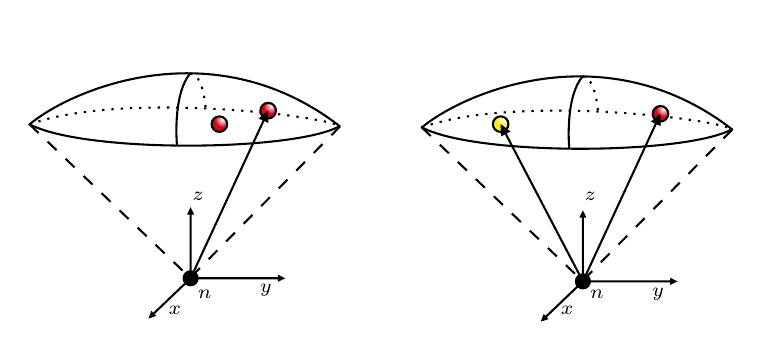
\begin{tikzpicture}[x=0.75pt,y=0.75pt,yscale=-1,xscale=1]
%uncomment if require: \path (0,300); %set diagram left start at 0, and has height of 300

%Curve Lines [id:da4791931175407256] 
\draw    (151.5,118.74) .. controls (171.93,101.66) and (240.27,72.66) .. (301.1,119.74) ;
%Shape: Boxed Bezier Curve [id:dp4920496949466463] 
\draw    (151.1,118.49) .. controls (164.79,125.97) and (199.55,129.31) .. (232.6,128.97) .. controls (244.14,128.85) and (255.47,128.28) .. (265.62,127.29) .. controls (281.63,125.73) and (294.73,123.1) .. (301.1,119.49) ;
%Shape: Circle [id:dp7943134273486183] 
\draw  [fill={rgb, 255:red, 0; green, 0; blue, 0 }  ,fill opacity=1 ] (225.73,192.89) .. controls (225.73,191.03) and (227.24,189.52) .. (229.11,189.52) .. controls (230.97,189.52) and (232.48,191.03) .. (232.48,192.89) .. controls (232.48,194.76) and (230.97,196.27) .. (229.11,196.27) .. controls (227.24,196.27) and (225.73,194.76) .. (225.73,192.89) -- cycle ;
%Straight Lines [id:da30325083519994966] 
\draw  [dash pattern={on 4.5pt off 4.5pt}]  (151.5,118.74) -- (229.11,192.89) ;
%Straight Lines [id:da47679977208221547] 
\draw  [dash pattern={on 4.5pt off 4.5pt}]  (301.1,119.74) -- (226.97,194.62) ;
%Straight Lines [id:da8140700773019683] 
\draw    (229.11,192.89) -- (271.68,192.88) ;
\draw [shift={(274.68,192.88)}, rotate = 179.98] [fill={rgb, 255:red, 0; green, 0; blue, 0 }  ][line width=0.08]  [draw opacity=0] (3.57,-1.72) -- (0,0) -- (3.57,1.72) -- cycle    ;
%Straight Lines [id:da47034622940515947] 
\draw    (229.09,161.63) -- (229.11,192.89) ;
\draw [shift={(229.09,158.63)}, rotate = 89.97] [fill={rgb, 255:red, 0; green, 0; blue, 0 }  ][line width=0.08]  [draw opacity=0] (3.57,-1.72) -- (0,0) -- (3.57,1.72) -- cycle    ;
%Straight Lines [id:da920216355207054] 
\draw    (210.97,210.22) -- (229.11,192.89) ;
\draw [shift={(208.8,212.29)}, rotate = 316.31] [fill={rgb, 255:red, 0; green, 0; blue, 0 }  ][line width=0.08]  [draw opacity=0] (3.57,-1.72) -- (0,0) -- (3.57,1.72) -- cycle    ;
%Curve Lines [id:da0920108067197728] 
\draw  [dash pattern={on 0.84pt off 2.51pt}]  (151.5,118.74) .. controls (195.95,102.58) and (294.93,114.66) .. (301.1,119.74) ;
%Shape: Circle [id:dp5035215917631497] 
\path  [shading=_r90b3jz8c,_yf8nxye1j] (262.72,112.13) .. controls (262.72,110.05) and (264.4,108.38) .. (266.47,108.38) .. controls (268.55,108.38) and (270.22,110.05) .. (270.22,112.13) .. controls (270.22,114.2) and (268.55,115.88) .. (266.47,115.88) .. controls (264.4,115.88) and (262.72,114.2) .. (262.72,112.13) -- cycle ; % for fading 
 \draw   (262.72,112.13) .. controls (262.72,110.05) and (264.4,108.38) .. (266.47,108.38) .. controls (268.55,108.38) and (270.22,110.05) .. (270.22,112.13) .. controls (270.22,114.2) and (268.55,115.88) .. (266.47,115.88) .. controls (264.4,115.88) and (262.72,114.2) .. (262.72,112.13) -- cycle ; % for border 

%Straight Lines [id:da8192496484494082] 
\draw    (229.11,192.89) -- (265.22,114.85) ;
\draw [shift={(266.47,112.13)}, rotate = 114.83] [fill={rgb, 255:red, 0; green, 0; blue, 0 }  ][line width=0.08]  [draw opacity=0] (5.36,-2.57) -- (0,0) -- (5.36,2.57) -- cycle    ;
%Curve Lines [id:da265617715955747] 
\draw    (222.5,128.58) .. controls (222.11,123.44) and (221.22,103.22) .. (229,94.08) ;
%Curve Lines [id:da3379607600300486] 
\draw  [dash pattern={on 0.84pt off 2.51pt}]  (229,94.08) .. controls (234.78,94.56) and (236.33,109) .. (236.33,111) ;
%Curve Lines [id:da8390561814886154] 
\draw    (340.5,120.24) .. controls (360.93,103.16) and (429.27,74.16) .. (490.1,121.24) ;
%Shape: Boxed Bezier Curve [id:dp2528126281927795] 
\draw    (340.1,119.99) .. controls (353.79,127.47) and (388.55,130.81) .. (421.6,130.47) .. controls (433.14,130.35) and (444.47,129.78) .. (454.62,128.79) .. controls (470.63,127.23) and (483.73,124.6) .. (490.1,120.99) ;
%Shape: Circle [id:dp023773067079900567] 
\draw  [fill={rgb, 255:red, 0; green, 0; blue, 0 }  ,fill opacity=1 ] (414.73,194.39) .. controls (414.73,192.53) and (416.24,191.02) .. (418.11,191.02) .. controls (419.97,191.02) and (421.48,192.53) .. (421.48,194.39) .. controls (421.48,196.26) and (419.97,197.77) .. (418.11,197.77) .. controls (416.24,197.77) and (414.73,196.26) .. (414.73,194.39) -- cycle ;
%Straight Lines [id:da7383701549266455] 
\draw  [dash pattern={on 4.5pt off 4.5pt}]  (340.5,120.24) -- (418.11,194.39) ;
%Straight Lines [id:da7816321005392438] 
\draw  [dash pattern={on 4.5pt off 4.5pt}]  (490.1,121.24) -- (415.97,196.12) ;
%Straight Lines [id:da11874025375985742] 
\draw    (418.11,194.39) -- (460.68,194.38) ;
\draw [shift={(463.68,194.38)}, rotate = 179.98] [fill={rgb, 255:red, 0; green, 0; blue, 0 }  ][line width=0.08]  [draw opacity=0] (3.57,-1.72) -- (0,0) -- (3.57,1.72) -- cycle    ;
%Straight Lines [id:da7975302078263008] 
\draw    (418.09,163.13) -- (418.11,194.39) ;
\draw [shift={(418.09,160.13)}, rotate = 89.97] [fill={rgb, 255:red, 0; green, 0; blue, 0 }  ][line width=0.08]  [draw opacity=0] (3.57,-1.72) -- (0,0) -- (3.57,1.72) -- cycle    ;
%Straight Lines [id:da24589489362880512] 
\draw    (399.97,211.72) -- (418.11,194.39) ;
\draw [shift={(397.8,213.79)}, rotate = 316.31] [fill={rgb, 255:red, 0; green, 0; blue, 0 }  ][line width=0.08]  [draw opacity=0] (3.57,-1.72) -- (0,0) -- (3.57,1.72) -- cycle    ;
%Curve Lines [id:da7218635165767303] 
\draw  [dash pattern={on 0.84pt off 2.51pt}]  (340.5,120.24) .. controls (384.95,104.08) and (483.93,116.16) .. (490.1,121.24) ;
%Shape: Circle [id:dp3595205172001702] 
\path  [shading=_dfo8mv0ol,_nifyjqsrp] (451.72,113.63) .. controls (451.72,111.55) and (453.4,109.88) .. (455.47,109.88) .. controls (457.55,109.88) and (459.22,111.55) .. (459.22,113.63) .. controls (459.22,115.7) and (457.55,117.38) .. (455.47,117.38) .. controls (453.4,117.38) and (451.72,115.7) .. (451.72,113.63) -- cycle ; % for fading 
 \draw   (451.72,113.63) .. controls (451.72,111.55) and (453.4,109.88) .. (455.47,109.88) .. controls (457.55,109.88) and (459.22,111.55) .. (459.22,113.63) .. controls (459.22,115.7) and (457.55,117.38) .. (455.47,117.38) .. controls (453.4,117.38) and (451.72,115.7) .. (451.72,113.63) -- cycle ; % for border 

%Straight Lines [id:da345731477933667] 
\draw    (418.11,194.39) -- (454.22,116.35) ;
\draw [shift={(455.47,113.63)}, rotate = 114.83] [fill={rgb, 255:red, 0; green, 0; blue, 0 }  ][line width=0.08]  [draw opacity=0] (5.36,-2.57) -- (0,0) -- (5.36,2.57) -- cycle    ;
%Shape: Circle [id:dp30312805210699323] 
\path  [shading=_6z78fwt66,_fal5ao0nl] (374.72,118.63) .. controls (374.72,116.55) and (376.4,114.88) .. (378.47,114.88) .. controls (380.55,114.88) and (382.22,116.55) .. (382.22,118.63) .. controls (382.22,120.7) and (380.55,122.38) .. (378.47,122.38) .. controls (376.4,122.38) and (374.72,120.7) .. (374.72,118.63) -- cycle ; % for fading 
 \draw   (374.72,118.63) .. controls (374.72,116.55) and (376.4,114.88) .. (378.47,114.88) .. controls (380.55,114.88) and (382.22,116.55) .. (382.22,118.63) .. controls (382.22,120.7) and (380.55,122.38) .. (378.47,122.38) .. controls (376.4,122.38) and (374.72,120.7) .. (374.72,118.63) -- cycle ; % for border 

%Straight Lines [id:da17088202492119942] 
\draw    (418.11,194.39) -- (379.87,121.28) ;
\draw [shift={(378.47,118.63)}, rotate = 62.39] [fill={rgb, 255:red, 0; green, 0; blue, 0 }  ][line width=0.08]  [draw opacity=0] (5.36,-2.57) -- (0,0) -- (5.36,2.57) -- cycle    ;
%Curve Lines [id:da9734970953245851] 
\draw    (411.5,130.08) .. controls (411.11,124.94) and (410.22,104.72) .. (418,95.58) ;
%Curve Lines [id:da4939755869812369] 
\draw  [dash pattern={on 0.84pt off 2.51pt}]  (418,95.58) .. controls (423.78,96.06) and (425.33,110.5) .. (425.33,112.5) ;
%Shape: Circle [id:dp23831061895101247] 
\path  [shading=_div3xhroj,_fhio33hpt] (239.22,118.63) .. controls (239.22,116.55) and (240.9,114.88) .. (242.97,114.88) .. controls (245.05,114.88) and (246.72,116.55) .. (246.72,118.63) .. controls (246.72,120.7) and (245.05,122.38) .. (242.97,122.38) .. controls (240.9,122.38) and (239.22,120.7) .. (239.22,118.63) -- cycle ; % for fading 
 \draw   (239.22,118.63) .. controls (239.22,116.55) and (240.9,114.88) .. (242.97,114.88) .. controls (245.05,114.88) and (246.72,116.55) .. (246.72,118.63) .. controls (246.72,120.7) and (245.05,122.38) .. (242.97,122.38) .. controls (240.9,122.38) and (239.22,120.7) .. (239.22,118.63) -- cycle ; % for border 



% Text Node
\draw (231.11,197) node [anchor=north west][inner sep=0.75pt]  [font=\scriptsize] [align=left] {$\displaystyle n$};
% Text Node
\draw (217,205) node [anchor=north west][inner sep=0.75pt]  [font=\scriptsize] [align=left] {$\displaystyle x$};
% Text Node
\draw (260.97,194) node [anchor=north west][inner sep=0.75pt]  [font=\scriptsize] [align=left] {$\displaystyle y$};
% Text Node
\draw (228.49,150) node [anchor=north west][inner sep=0.75pt]  [font=\scriptsize] [align=left] {$\displaystyle z$};
% Text Node
\draw (420.11,197) node [anchor=north west][inner sep=0.75pt]  [font=\scriptsize] [align=left] {$\displaystyle n$};
% Text Node
\draw (406,205) node [anchor=north west][inner sep=0.75pt]  [font=\scriptsize] [align=left] {$\displaystyle x$};
% Text Node
\draw (449.97,196) node [anchor=north west][inner sep=0.75pt]  [font=\scriptsize] [align=left] {$\displaystyle y$};
% Text Node
\draw (417.49,150) node [anchor=north west][inner sep=0.75pt]  [font=\scriptsize] [align=left] {$\displaystyle z$};


\end{tikzpicture}
